%% Exercice 2

%\ExoSpecs{\TTBF{CalculTVA.sh}}{\TTBF{\RenduDir/src/exo1/}}{750}{640}{\TTBF{write}}
\ExoSpecsCustom{\TTBF{GraphStats.py}}{\TTBF{\RenduDir/src/}}{750}{640}{Modules recommandés}{\TTBF{sys}, \TTBF{datetime}, \TTBF{csv}, \TTBF{pandas}, \TTBF{matplotlib.pyplot}}
%, \TTBF{plotly.graph\_objects}}
%{\TTBF{math.floor}, \TTBF{math.ceil}, \TTBF{random.random}}

\vspace*{0.7cm}

\noindent \ExoObjectif{Le but de l'exercice est d'écrire une classe faisant des appels aux APIs, lisant un CSV, et produisant des diagrammes statistiques.}
%Optionnellement, une carte géographique avec placement par longitude et latitude pourra être réalisée.}

\bigskip

\noindent Vous devrez réutiliser une partie du code écrit dans l'exercice 1, mais de façon plus précise.

\bigskip

\noindent La documentation pour les différents modules externes est accessibles via ces liens :

\begin{itemize}
\item DateTime : \url{https://docs.python.org/fr/3/library/datetime.html}
\item CSV : \url{https://docs.python.org/fr/3/library/csv.html}
\item Pandas : \url{https://pandas.pydata.org/docs/user\_guide/index.html}
\item Matplotlib : \url{https://matplotlib.org/stable/tutorials/introductory/usage.html}
%\item ScatterGeo : \url{https://plotly.com/python-api-reference/generated/plotly.graph\_objects.Scattergeo.html}
\end{itemize}

\bigskip

\begin{figure}[!h]
    \centering
    \begin{subfigure}[b]{0.45\textwidth}
        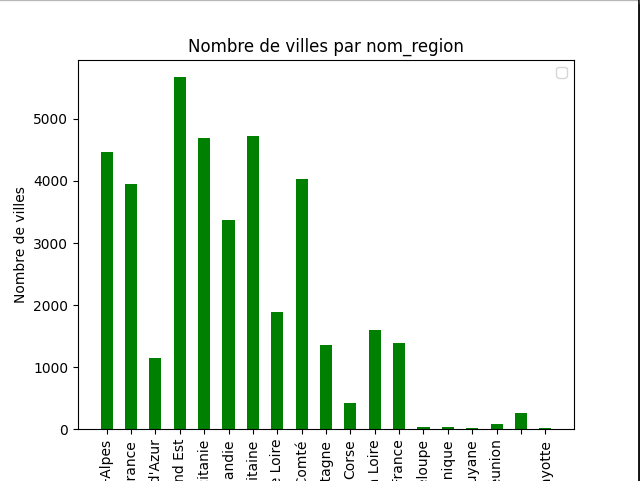
\includegraphics[width=\textwidth]{images/Exemple-Histogramme.png}
    \end{subfigure}
    \begin{subfigure}[b]{0.45\textwidth}
        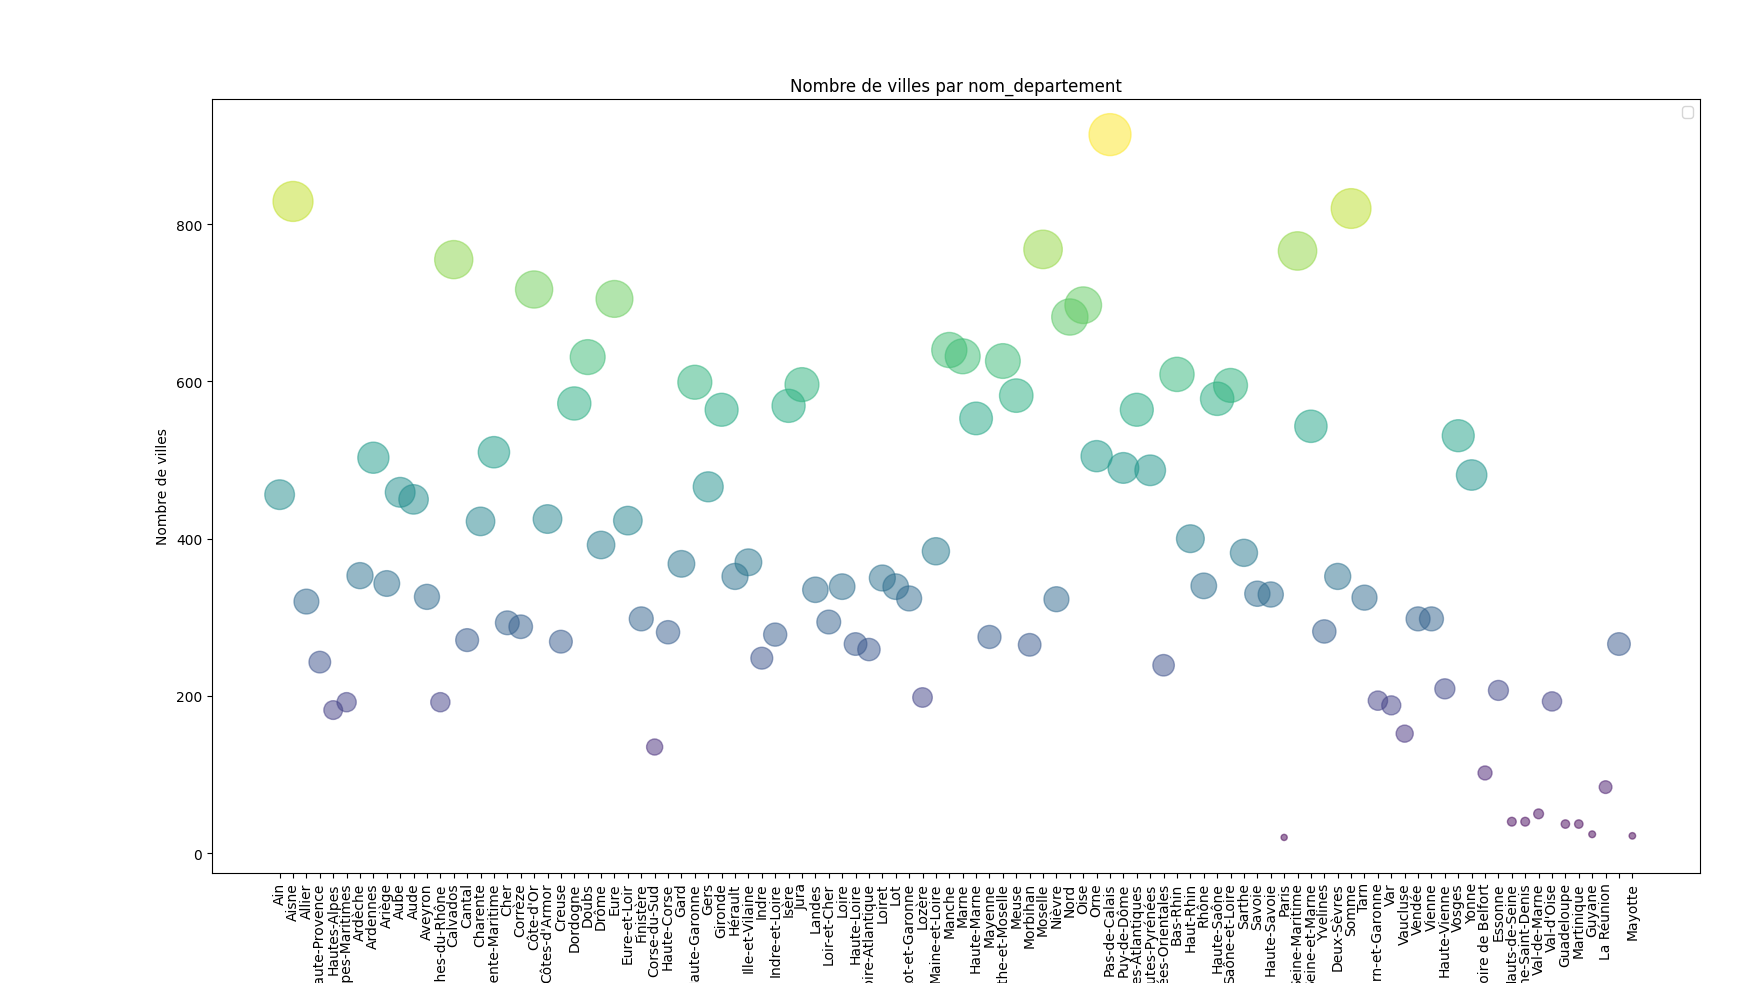
\includegraphics[width=\textwidth]{images/Exemple-Scatter.png}
    \end{subfigure}
    \caption{Exemples de graphiques statistiques avec Matplotlib}
    \label{Exemple-1-Graph-Matplotlib}
\end{figure}


%\begin{figure}[!h]
%    \centering
%%    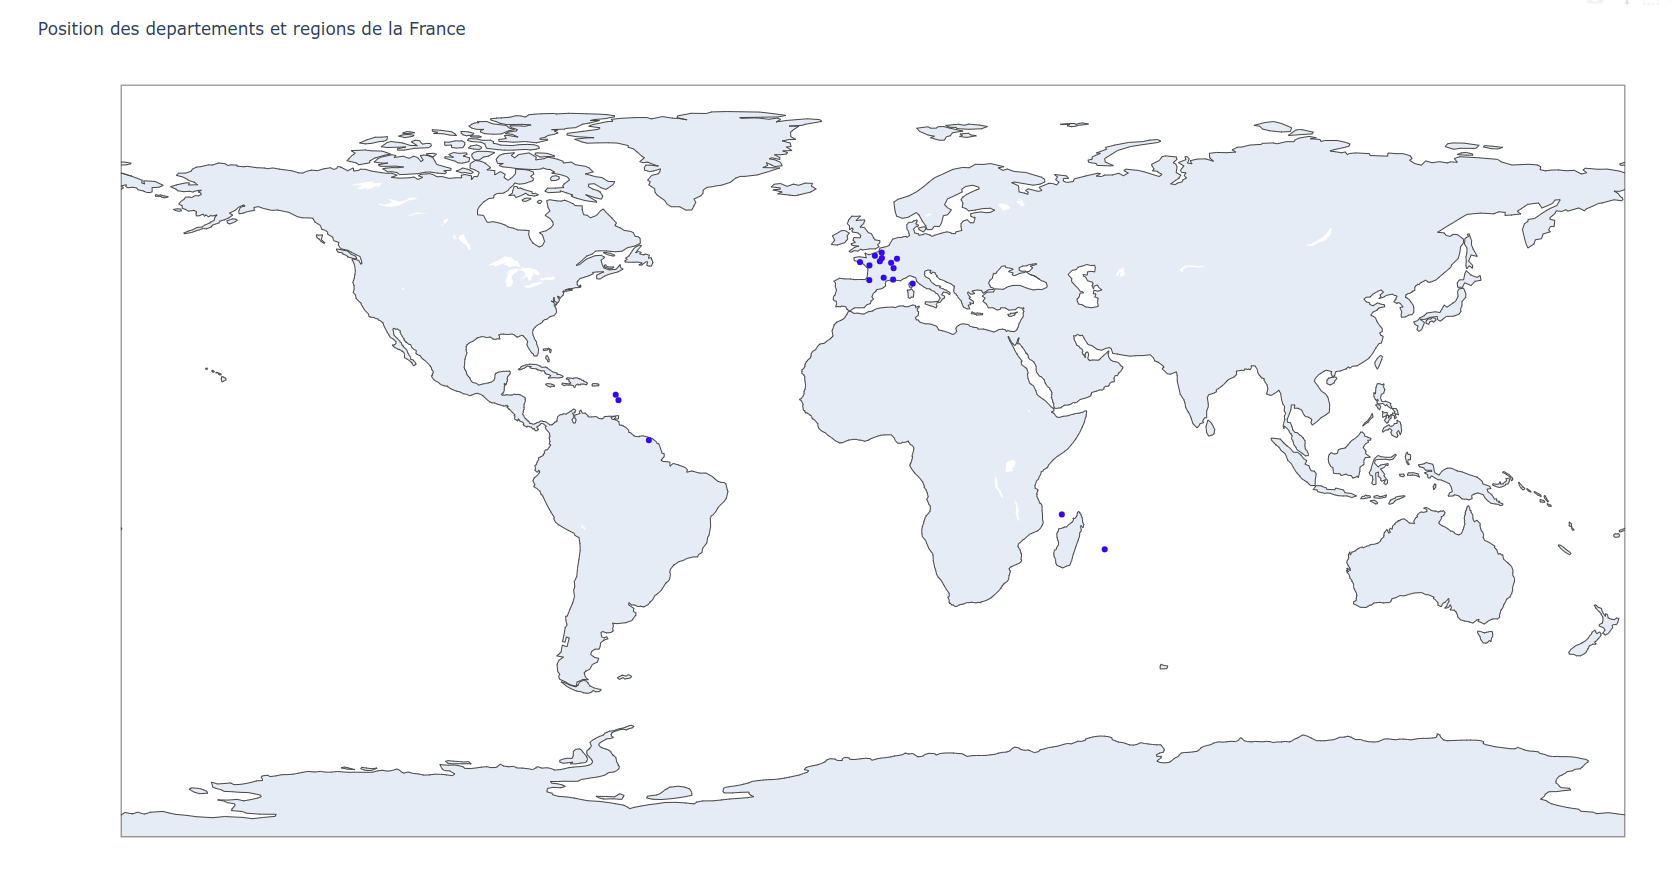
\includegraphics[width=\textwidth]{images/Exemple-CarteMondiale.png}
%    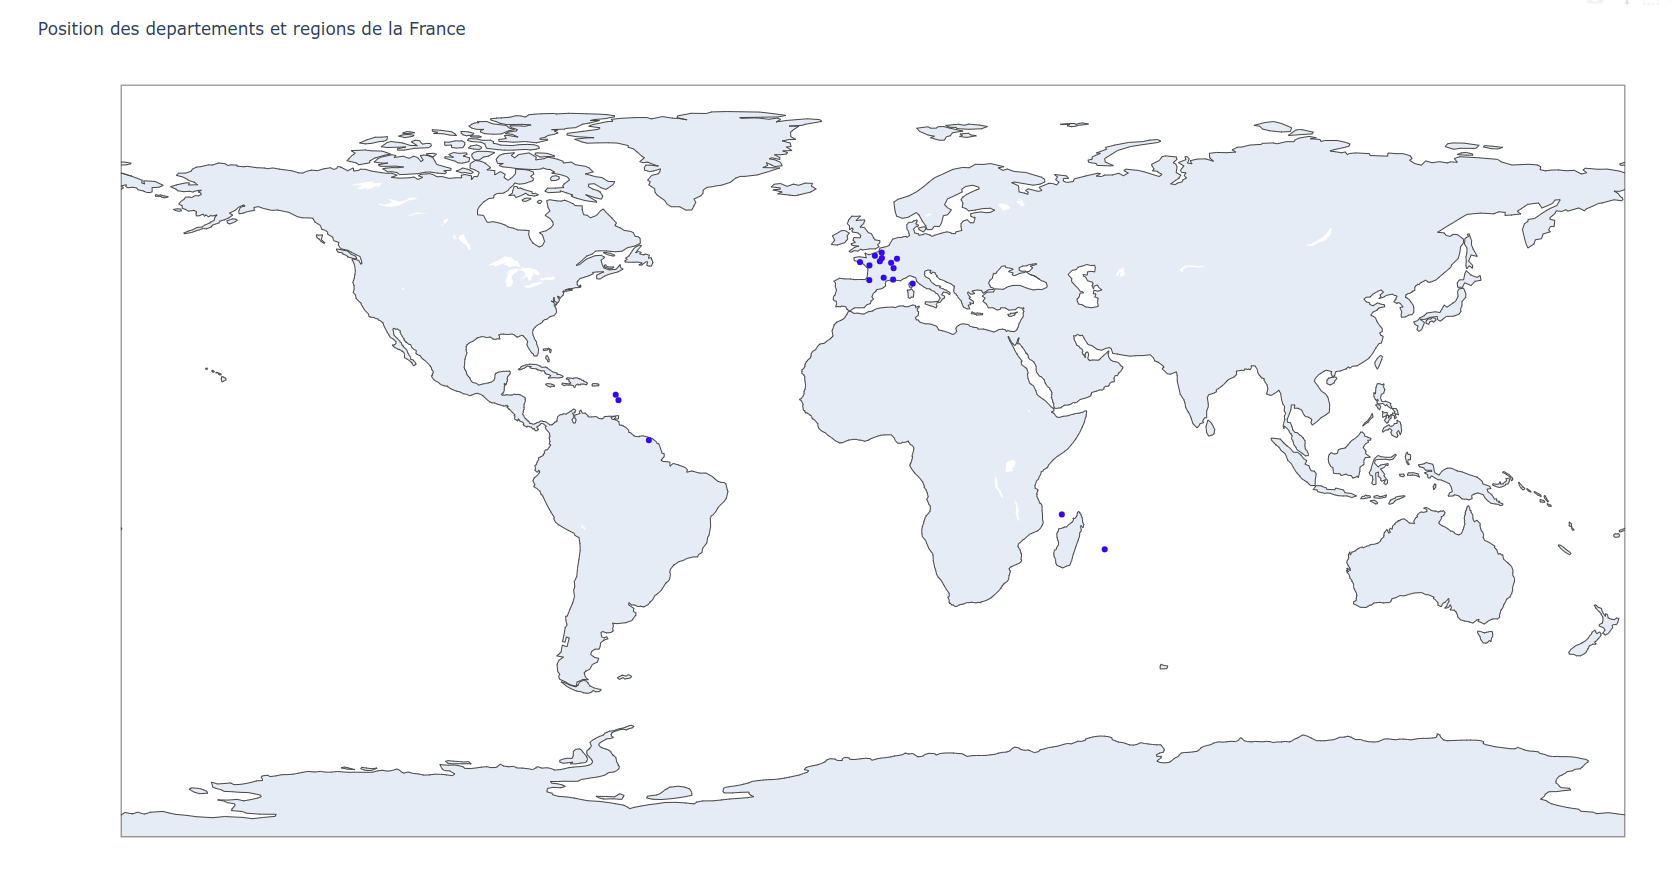
\includegraphics[width=0.6\textwidth]{images/Exemple-CarteMondiale.png}
%    \caption{Exemples de carte géographique avec ScatterGeo}
%    \label{Exemple-2-Geo-Map}
%\end{figure}

\bigskip

\noindent Les différents appels aux APIs publiques que vous avez réalisés vous ont permis de récupérer les données brutes, et de les afficher de façon très rudimentaires dans le terminal.
Néanmoins, un affichage graphique améliorera non seulement l'esthétique, mais également la lisibilité et la capacité à comprendre les informations contenues dans les données.

\medskip

\noindent Afin d'étendre un peu plus les analyses, vous devrez récupérer un fichier CSV en ligne et le lire pour en tirer des informations que vous croiserez avec les données sur la population.
Le fichier CSV contient une liste de villes et leur département ainsi que leur région d'appartenance.
Il peut être directement fourni en paramètre aux modules \TTBF{csv} et \TTBF{Pandas} sans être téléchargé préalablement.
Celui-ci est accessible ici : \url{https://www.data.gouv.fr/fr/datasets/r/dbe8a621-a9c4-4bc3-9cae-be1699c5ff25}

\bigskip

\noindent Vous devez implémenter les fonctions décrites plus bas, si nécessaire en déclarant vos propres fonctions.
Ce code sera testé en étant lui-même appelé par un autre script, vous devez donc absolument respecter les prototypes décrits ici.

%\bigskip
%\newpage

\bigskip


\subsubsection*{Fonction \TTBF{main()}}

\noindent Cette fonction sera celle appelée lorsque le script est lancé.
Elle ne prend pas de paramètre, mais elle lit les arguments donnés en ligne de commande puis instancie la classe GraphStat et appelle la méthode \TTBF{ProcessAndDraw()}.
Si tout se passe bien, le script doit renvoyer \TTBF{0}.
Deux paramètres, dont le deuxième est optionnel, doivent être testés :

\begin{enumerate}
\item Le premier argument est l'année de recensement qui sera demandée à l'API des populations millésimées par département.

\item Le deuxième argument est le format de graphique attendu.
  \begin{itemize}
  \item L'argument \TTBF{bar} indique que l'utilisateur souhaite un diagramme en barres (le format \og \textit{bâtonnets} \fg{}, ou \textit{bar chart} en anglais).
  \item L'argument \TTBF{pie} indique que l'utilisateur souhaite un diagramme circulaire (le format \og \textit{camembert} \fg{}, ou \textit{pie chart} en anglais).
  \item Si aucun de ces choix n'est sélectionné, alors l'option \TTBF{bar} sera sélectionnée par défaut.
  \end{itemize}
\end{enumerate}

\bigskip

\noindent Si le premier argument (année du recensement) est donné mais n'est pas un entier positif entre \TTBF{1800} et l'année courante, le script doit se terminer en renvoyant \TTBF{-1} et en écrivant :

\bigskip

\lstset{language=sh}
\begin{lstlisting}[frame=single]
$ python GraphStats.py 42 bar
Year must be greater than "1800" and at most current year (2023)
./GraphStats.py year [default:bar | pie]
$ echo $?
255
\end{lstlisting}



\noindent Si un deuxième argument (format du graphique) est donné mais n'est ni \TTBF{bar} ni \TTBF{pie}, le script doit se terminer en renvoyant \TTBF{-2} et en écrivant :

\bigskip

\lstset{language=sh}
\begin{lstlisting}[frame=single]
$ python GraphStats.py 2019 wololooo
Graphic format must be "bar" or "pie" (or can be omitted)
./GraphStats.py year [default:bar | pie]
$ echo $?
254
\end{lstlisting}


\clearpage


\noindent Si les deux arguments sont problématiques, celui de l'année prime sur celui du format de graphique :

\bigskip

\lstset{language=sh}
\begin{lstlisting}[frame=single]
$ python GraphStats.py 4 chan
Year must be greater than "1800" and at most current year (2023)
./GraphStats.py year [default:bar | pie]
$ echo $?
255
\end{lstlisting}


\noindent Enfin, si le premier argument est un \TTBF{-h}, \TTBF{--help}, ou qu'il n'y a aucun argument, le script doit afficher ce message et renvoyer \TTBF{0} sans rien faire d'autre :

\bigskip

\lstset{language=sh}
\begin{lstlisting}[frame=single]
$ python GraphStats.py -h
./GraphStats.py year [default:bar | pie]
$ echo $?
0
\end{lstlisting}

\lstset{language=sh}
\begin{lstlisting}[frame=single]
$ python GraphStats.py --help
./GraphStats.py year [default:bar | pie]
$ echo $?
0
\end{lstlisting}

\lstset{language=sh}
\begin{lstlisting}[frame=single]
$ python GraphStats.py
./GraphStats.py year [default:bar | pie]
$ echo $?
0
\end{lstlisting}


%\bigskip
\clearpage

\subsubsection*{Classe \TTBF{GraphStat}}

\noindent Cette classe permet de faire les appels aux APIs, calculer les ratios, et dessiner les graphiques associés.
Elle contient au moins ces méthodes et attributs :

\bigskip

\lstset{language=python}
\begin{lstlisting}[frame=single]
__init__(self, year, graph_type)
__GetPopulation(self, year)
__GetVilles(self)
__BuildPopulationDict(self, Dict_API)
__BuildCityDict(self, data)
__BuildDepartementDict(self, data)
__CalculateStats(self, Dict_Pop, Dict_Cities)
__DrawBar(self, Dict_Ratio, Dict_ID_Dept, asc=False)
__DrawPie(self, Dict_Ratio, Dict_ID_Dept, asc=False)
ProcessAndDraw(self)

year
graph_type
\end{lstlisting}


\bigskip


\subsubsection*{\TTBF{\_\_init\_\_(self, year, graph\_type)}}

\noindent Cette méthode récupère les paramètres fournis par la fonction \TTBF{main()} et les assigne aux attributs \TTBF{year} et \TTBF{graph\_type} contenus dans la classe \TTBF{GraphStat}.
Attention, cette méthode n'exécute rien d'autre.


\bigskip


\subsubsection*{\TTBF{\_\_GetPopulation(self, year)}}

\noindent Cette méthode exécute l'appel à l'API pour obtenir la \textit{population totale} par département pour l'année donnée en paramètre, puis elle renvoie la réponse donnée par l'API.
L'année correspond à l'attribut/champs \TTBF{strat\_year} de l'API.
L'URL de l'API est la suivante : \url{https://public.opendatasoft.com/explore/dataset/demographyref-france-pop-legale-departement-millesime}

\noindent Si la réponse de l'API est vide, cette méthode termine le script en renvoyant \TTBF{-3} et en écrivant le message suivant :

\bigskip

\lstset{language=sh}
\begin{lstlisting}[frame=single]
$ python GraphStats.py 2000 bar
Sadly, no data was available for year "2000".
Try again with another date.
$ echo $?
253
\end{lstlisting}


\bigskip


\subsubsection*{\TTBF{\_\_GetVilles(self)}}

\noindent Cette méthode récupère le fichier CSV depuis l'API publique, puis elle renvoie le \textit{dataframe} qui en est extrait (dans le cas d'utilisation du module \textit{Pandas}) ou la matrice représentant le CSV (dans le cas d'utilisation du module \textit{csv}).

\noindent L'URL pour accéder au dataset est la suivante : \url{https://www.data.gouv.fr/fr/datasets/r/dbe8a621-a9c4-4bc3-9cae-be1699c5ff25}


\bigskip


\subsubsection*{\TTBF{\_\_BuildPopulationDict(self, Dict\_API)}}

\noindent Cette méthode construit un dictionnaire dont les clés sont les codes des départements, et les valeurs sont la population totale de chaque département.
Le paramètre d'entrée est le dictionnaire de données renvoyée par l'API traitant de la démographie.


\bigskip


\subsubsection*{\TTBF{\_\_BuildCityDict(self, data)}}

\noindent Cette méthode construit un dictionnaire dont les clés sont les codes des départements, et les valeurs sont la quantité de villes pour chaque département.
Le paramètre d'entrée est le tableau contenant la liste des villes par département (soit un \textit{dataframe} si vous avez utilisé le module \textit{Pandas}, soit une matrice si vous avez utilisé le module \textit{csv}).


\bigskip


\subsubsection*{\TTBF{\_\_BuildDepartementDict(self, data)}}

\noindent Cette méthode construit un dictionnaire dont les clés sont les codes des départements, et les valeurs sont les noms complets de chaque département.
Le paramètre d'entrée peut aussi bien être le dictionnaire de données renvoyée par l'API traitant de la démographie, ou le tableau contenant la liste des villes par département.


\bigskip


\subsubsection*{\TTBF{\_\_CalculateStats(self, Dict\_Pop, Dict\_Cities)}}

\noindent Cette méthode calcule le ratio entre la population de chaque département et le nombre de villes contenus dans chacun d'entre eux.
La fonction prend en premier paramètre un dictionnaire dont les clés sont les codes des départements et les valeurs sont la population contenue dans chacun d'eux, et le deuxième paramètre est un dictionnaire dont les clés sont les codes des départements et les valeurs sont la quantité de villes dans chacun des départements.

\noindent La méthode doit renvoyer un dictionnaire dont les clés sont les codes des départements, et les valeurs sont les ratios.


\bigskip


\subsubsection*{\TTBF{\_\_DrawBar(self, Dict\_Ratio, Dict\_ID\_Dept, [asc=False])}}

\noindent Cette méthode dessine le diagramme en barres appliqué aux données en paramètres.

\noindent Le premier dictionnaire en paramètre contient en clés les codes des départements et en valeurs les ratios des population/villes.
Le deuxième dictionnaire en paramètre contient en clés les codes des départements et en valeurs les noms complets des départements.
Le troisième paramètre est optionnel et sert à indiquer si l'on souhaite afficher les 10 ratios les plus élevés (en ordre décroissant), ou les 10 ratios les plus faibles (en ordre croissant).

\noindent Pour ce graphique, la couleur des barres doit être \TTBF{green} et leur largeur de \TTBF{0.5}.

\noindent Le diagramme à afficher doit indiquer en hauteur le ratio, et à la base les noms complets des départements.


\bigskip


\subsubsection*{\TTBF{\_\_DrawPie(self, Dict\_Ratio, Dict\_ID\_Dept, [asc=False])}}

\noindent Cette méthode dessine le diagramme circulaire appliqué aux données en paramètres.

\noindent Le premier dictionnaire en paramètre contient en clés les codes des départements et en valeurs les ratios des population/villes.
Le deuxième dictionnaire en paramètre contient en clés les codes des départements et en valeurs les noms complets des départements.
Le troisième paramètre est optionnel et sert à indiquer si l'on souhaite afficher les 5 ratios les plus élevés, ou les 5 ratios les plus faibles.

\noindent Afin d'obtenir un diagramme comparant correctement les ratios de l'ensemble de la base de données, vous afficherez en gris dans un seul secteur l'ensemble des ratios non pris en compte, et les 5 sélectionnés (les plus élevés ou les plus faibles) en couleurs :

\begin{table}[ht!]
  \centering
\begin{tabular}{c c}
  \begin{minipage}{0.45\textwidth}

\begin{enumerate}
\item rouge pour le plus grand,
\item orange pour le suivant,
\item jaune pour le suivant,
\end{enumerate}

  \end{minipage}
&
  \begin{minipage}{0.45\textwidth}

\begin{enumerate}
\setcounter{enumi}{4}
\item vert pour le suivant,
\item et bleu pour le dernier.
\end{enumerate}

\phantom{Test.}

  \end{minipage}
\end{tabular}
\end{table}


\noindent Le diagramme à afficher doit indiquer les ratios et les noms complets des départements.


\bigskip


\subsubsection*{\TTBF{ProcessAndDraw(self)}}

\noindent Cette méthode est la seule méthode publique (au sens POO) : c'est celle-ci qui doit être appelée par le code externe pour déclencher la récupération des données auprès des APIs externes, faire tous les calculs de ratios et préparer les dictionnaires, puis choisir la bonne méthode pour dessiner le graphique de sortie à partir des attributs enregistrés dans la classe.
